\begin{figure}
  \centering
  \begin{subfigure}[t]{0.42\textwidth}
    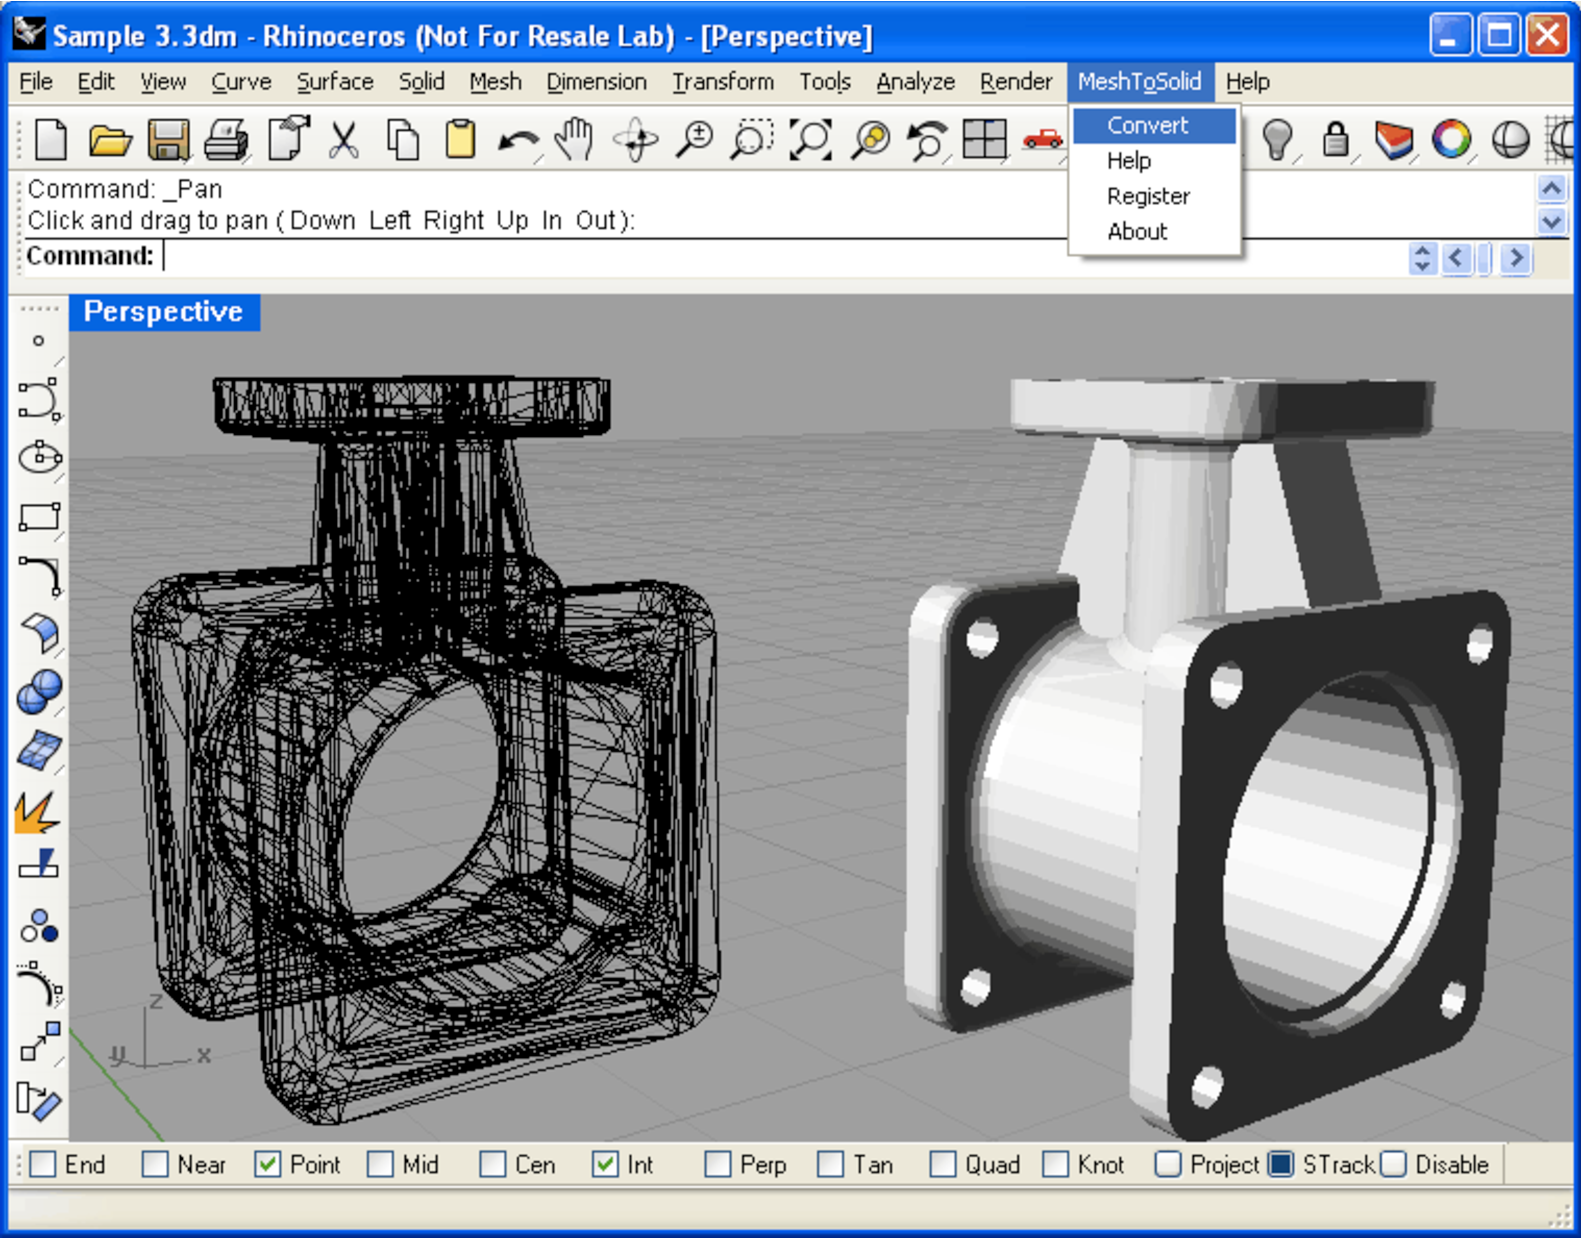
\includegraphics[width=\linewidth]{img/rhino3d-screenshot.pdf}
    \caption{Rhino 3D modeling software.}
    \label{fig:rhino3d-screenshot}
  \end{subfigure}
  \hspace{1cm} % spacing, do what you need
  \begin{subfigure}[t]{0.42\textwidth}
    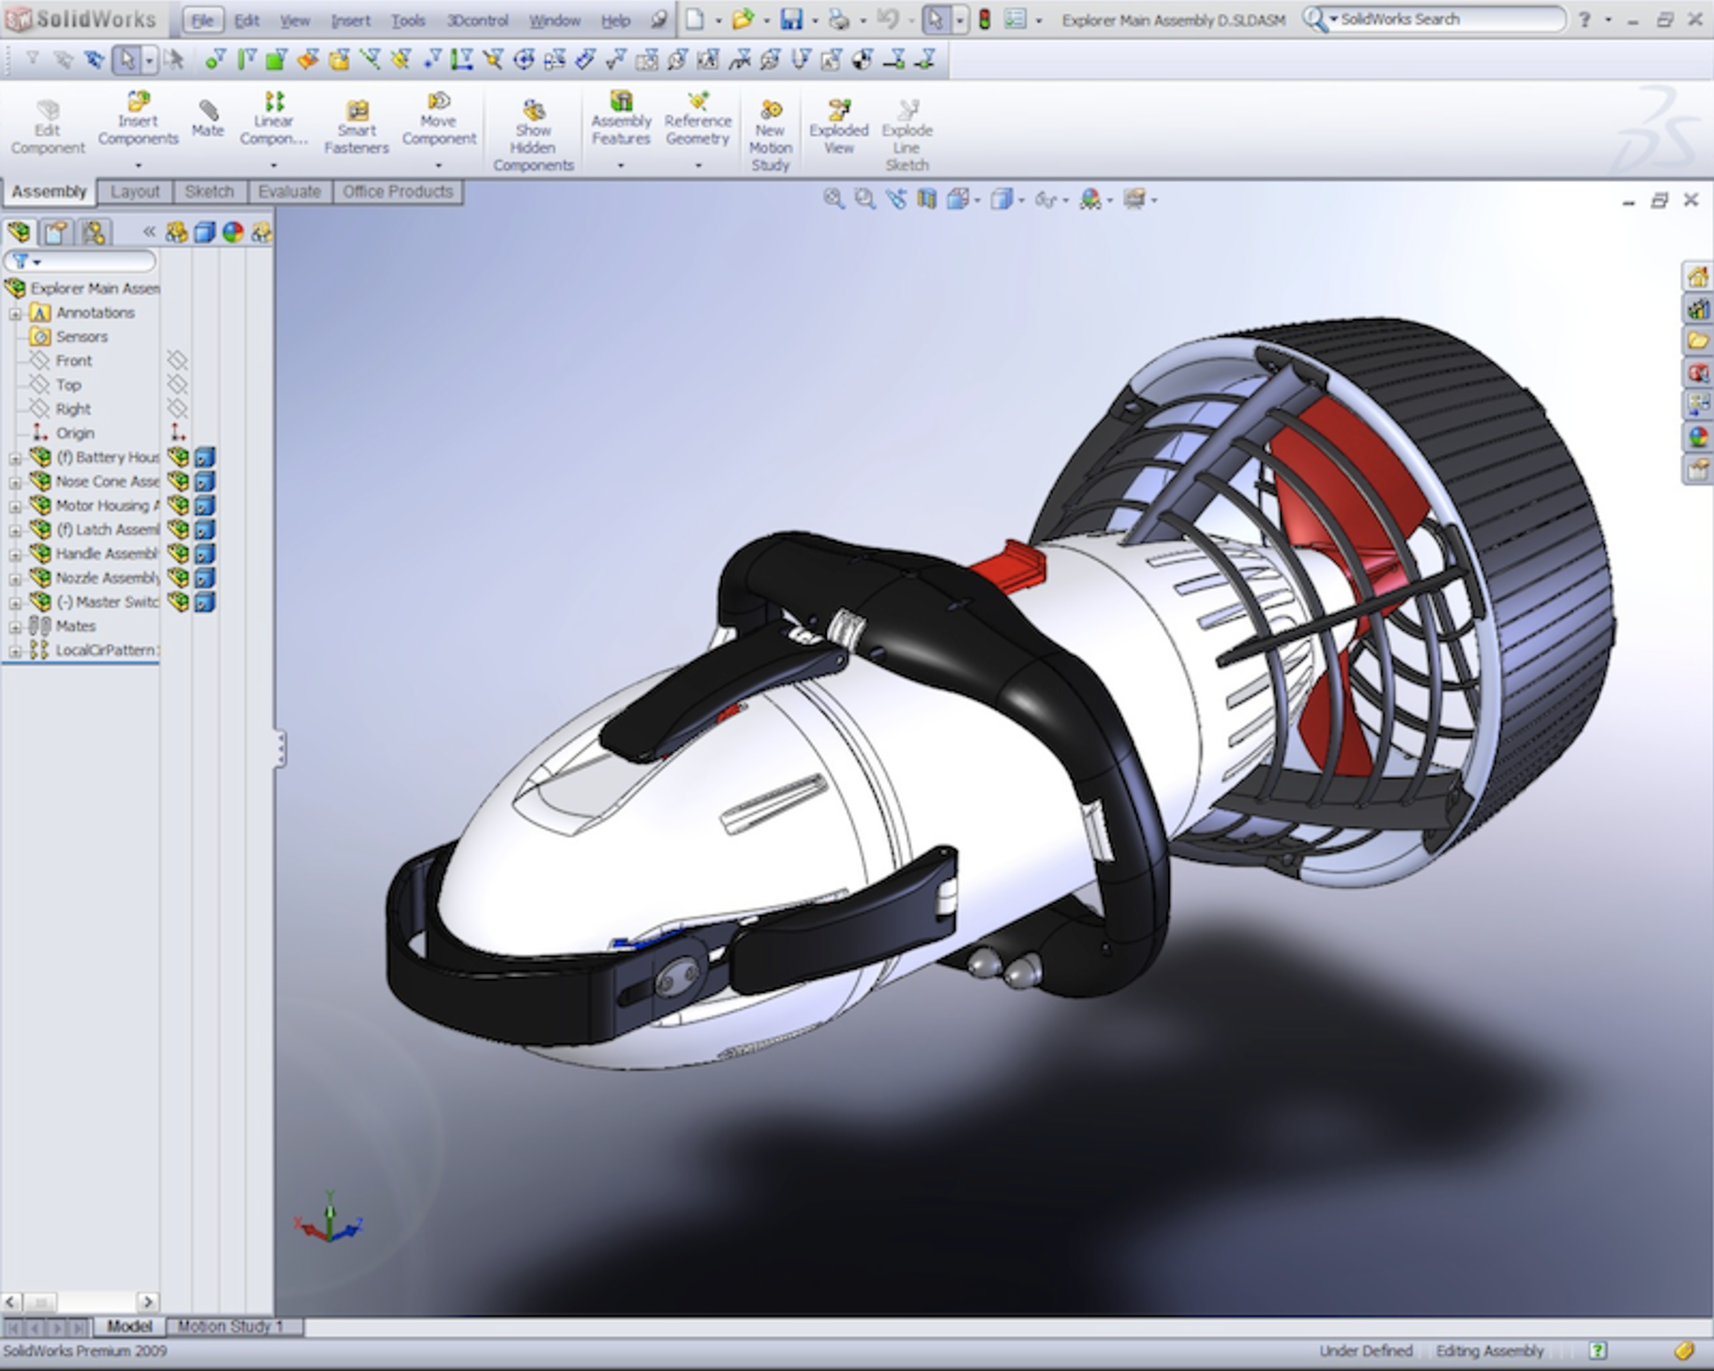
\includegraphics[width=\linewidth]{img/solidworks-screenshot.pdf}
    \caption{Solidworks modeling tool.}
    \label{fig:solidworks-screenshot}
  \end{subfigure}
  \caption[Advanced 3D CAD Software]{Rhino 3D and Solidworks are two commonly used 3D modeling tools and are often used by skilled users for various rapid fabrication purposes, including laser cutting.}
  \label{fig:cad-screenshots}
\end{figure}
